\chapter{Browsers y Estado del Arte}
\label{chap4:EA}

\section{Arquitectura de Referencia del Browser y Patrones}
\label{chap3:ArqRefBrowandPatt}

%Decir: "este trabajo es basado en la metodología de Fernandez \cite{Hashizume2014Reference} usando patrones en la construcción de la arquitectura de referencia"

\subsection{Método}
El primer paso para realizar el estado del arte con respecto a este punto fue realizar una búsqueda ordenada y a través de string de búsqueda dentro de web engines y librerías digitales conocidas. Se utilizaron las siguientes plataformas para buscar documentación al respecto:
\begin{itemize}
    \item Google, usando \textit{google dorks} para filtrar resultados
    \item Scopus y Google Scholar, usando string de búsqueda y operadores booleanos para filtrar resultados.
\end{itemize}

Para aquellos buscadores donde era posible usar operadores booleanos también se trató de filtrar el contenido para que pudiera mostrar resultados relacionados a: \textit{Browser} y \textit{Reference Architecture}. Sin embargo los resultados fueron bastante pobres. Desafortunadamente hasta la fecha no existen muchos trabajos relacionados a la construcción de una Arquitectura de Referencia para el Browser. Dado que la búsqueda no entregó muchos resultados, se procedió a hacer un \textit{forward snowballing} con el único paper que creemos entrega información similar a lo que se buscaba. Sin embargo, tampoco encontramos tanta información.

\subsection{Lo encontrado}
%larrondo
En Larrondo-Petrie et. al \cite{535061} se realiza un análisis del web browser, con el fin de obtener un Modelo de Dominio, un Modelo de Objetos y un \textit{Feature Tree} que describiera la estructura y funcionalidad entregada comúnmente por los Web Browser. El dominio, según explica el trabajo, es un set distintivo de objetos que se comportan de acuerdo a reglas y política que caracterizan el Dominio. El Análisis de Dominio es realizado para identificar dominios y cómo estos interactuan con otros. La metodología usada para obtener los Dominios es el \textit{Object Oriented Analyis}. Además de identificar, se clasifican estos dominios de acuerdo a su rol en el sistema terminado como: Dominio de Aplicación, Dominio de Servicio, Dominio de Arquitectura y Dominio de Implemntación. El Modelo de Objetos sirve para entregar más detalles, un resumen general de las Entidades del Web Browser y sus relaciones. El Feature Tree pretende entregar detalles sobre los aspectos funcionales de la aplicación. El Modelo planteado, śegún el artículo, debería ser útil para los Desarrolladores de Software que construyen \textbf{Aplicaciones Web basadas en el uso del Browser}.  Este estudio se encuentra bastante lejos de lo que se quiere hacer en este trabajo, pero sirve para obtener un transfondo de lo que sucede en el Web Browser, aún cuando la información esté muy desactualizada.

% preprint-grosskurth-browser-archevol y 2005-grosskurth-browser-refarch

En el trabajo de Grosskurth et al. \cite{2005-grosskurth-browser-refarch, preprint-grosskurth-browser-archevol} se utiliza una herramienta de ingeniería inversa, para obtener una arquitectura de referencia de muy alto nivel en base a dos navegadores open-source: Mozilla y Konqueror. Lo obtenido captura los subsistemas fundamentales comunes a los sistemas del mismo dominio, así como las relaciones entre estos subsistemas. En esta arquitectura se identifican los siguientes subcomponentes: Interfaz Usuaria, Persistencia de Datos, Browser Engine, Rendering Engine, Networking, Interprete de Javascript, XML Parser y Display Backend. Se menciona que estos componentes están estrechamente integrados (high coupling) con el Rendering Engine, lo cuál tiene sentido en la arquitectura monoproceso que poseen Mozilla y Konqueror; es una decisión de diseño muy común en los Browser de la época. Al identificar estos componentes, se comenta que ésto podría servir tanto en el diseño y durante la mantención de un sistema, pues mejora el entendimiento de un sistema al ayudar a analizar los trade-off entre diferentes opciones de diseño; o también puede servir como un template para obtener nuevos diseños. Una vez obtenida la arquitectura conceptual, se inició una evaluación de ésta al comparar las arquitecturas concretas de cada browser open-source, extraídas desde el código fuente, para ver que tanto el modelo conceptual era cercano a la realidad; la constante comparación permitió ademas refinar Arquitectura de Referencia. Los browsers usados para validar fueron: Epiphany, Safari, Lynx, Mosaic y Firefox. Si bien la arquitectura entregada entrega bastante información a alto nivel, no desarrolla más que esa capa de abstracción, además parece ser que depende también de la implementación usada en la herramienta de ingeniería inversa. 


%Godfrey2000
En el documento \cite{Godfrey2000} realizado en el año 2000, se describe la experiencia realizada al extender el rabajo del proyecto TAXFORM. Usando PBS, una herramienta de Ingeniería Inversa, se extrajo la arquitectura de software del Navegador Mozilla, con el objetivo de entender la estructuración de sus componentes; además de crear vistas arquitecturales de alto nivel del sistema. El modelo arquitectónico obtenido contiene 11 subsistemas de alto nivel, de éstos los que más se destacaron fuer el \textit{HTML Layout}, la implementación de herramientas y el código de la interfaz de usuario. En el año en que se lleva a cabo este estudio (2000), se menciona que la arquitectura ha decaído significativamente en muy poco tiempo, o su arquitectura no fue planificada cuidadosamente desde el comienzo; parte de lo anterior, el autor cree que es secuela de la \textit{Guerra de Navegadores}. Si bien el trabajo ayuda a entender un poco la estructura detrás del navegador, este trabajo es muy antiguo y la versión más actual del navegador ha cambiado bastante. Además lamentablemente, el enfoque de este estudio no es intentar entender lo que hace cada subsistema, si no que es la implementación de la herramienta misma para obtener la arquitectura de software del browser seleccionado.

%Lwin2009 - Agent Based Web Browser
En \cite{Lwin2009} se propone un Browser llamado Anfel SOFT, donde gracias al uso de Inteligencia Artificial, crea agentes que permiten mejorar la experiencia del usuario. El trabajo asegura que el browser será capaz de aprender el comportamiento de navegación del usuario, y guiará al usuario en su navegación para que esta sea lo más efectiva posible. El paper obtiene los subsistemas que se pueden encontrar en un browser de la misma manera que lo realiza \cite{2005-grosskurth-browser-refarch}. Si bien la arquitectura que muestra refleja parte de lo visto en los 3 browsers escogidos en este estudio, no da detalles acerca de cada subsistema identificado. Además la arquitectura de Referencia que entrega es la misma vista en \cite{2005-grosskurth-browser-refarch, preprint-grosskurth-browser-archevol} y a pesar que identifica otros posibles componentes, no agrega nada nuevo.

Podemos ver en los trabajos que algunos construyen una Arquitectura de Referencia basada en técnicas de Ingeniería Inversa. En cada uno de ellos el trabajo ha sido a muy alto nivel y la descripción de los subcomponetes del sistema es mínima. Si bien explican las relaciones entre éstos, no dan un mayor entendimiento en como se comportan en ciertas situaciones. En este trabajo se espera profundizar un poco más en la abstracción obtenida, incluyendo información de tanto los casos de uso del Browser como las actividades que se realizan con otros usuarios. Desafortunadamente para esta memoria no existe mucha literatura sobre el desarrollo de una Arquitectura de Referencia del Browser, y de lo que hay el trabajo más actual es el realizado por \cite{Lwin2009} en el año 2009.


\section{Google Chrome y Google Chromium}
    \label{chap3:GC}
    La misión de Google es organizar la información del mundo y lograr que sea útil y accesible para todo el mundo. Esta gran empresa partió como un búscador y rápidamente llegó a ser dueño de la mayor parte de búsquedas del mercado. Tiene servicios de almacenamiento en la nube, correo electrónico, \textit{e-wallet} y otros más. Google ha sido responsable por la construcción del Navegador Web \textbf{Google Chrome} y \textit{Google Chromium}. En el 2008, Google liberó gran parte del código de Chrome bajo el proyecto de nombre Google Chromium, el cuál es open-source que permitiría a desarrolladores \textit{third-party}, estudiar el código fuente y ayudar en la implementación para las plataformas Linux y OS X. La diferencia entre Chrome y Chromium son: actualizaciones automáticas y Adobe Flash integrado (aunque éste último ya se está cambiando el uso por HTML5). En  \cite{EvolutionofWeb} se menciona que este Navegador ha sido el último que ha salido y se llevado una gran parte del mercado \cite{statBrow}.

    La arquitectura de Chrome o Chromium se basa principalmente en dos módulos: el Browser Kernel y el Rendering Engine, cómo se puede ver en la Figura \ref{fig:archG}.

    \begin{figure}[h!t]
        \centering
        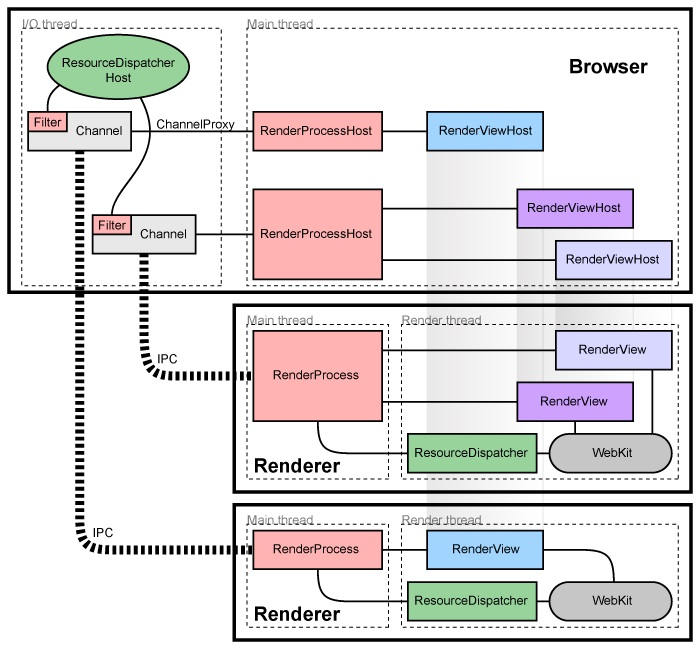
\includegraphics[scale=0.5]{figures/archGC.jpg}
        \caption{Architectura Multi procesos de Google Chrome. Fuente: \cite{multiProcGC}}
        \label{fig:archGC}
    \end{figure}

    Én la documentación de Google Chromium \cite{multiProcGC}, que es base para Google Chrome, afirma que la arquitectura soporta para cada tab un proceso nuevo, de manera de hacer al Browser más robusto y modularizar el sistema para evitar ciertas amenazas de seguridad. El proceso principal es llamado \textit{Browser Process/Kernel/Engine} y se encarga de la \textit{User Interface}, manejo de las tabs y los procesos de los \textit{plug-in}. Cada tab es asociado a un Rendering Engine, éstos tienen restricciones de acceso (\textit{Sandoboxing}) a los demas y al sistema, lo que permite que exista una protección de la memoria y un control de acceso. Google Chrome expone en \cite{reis2009browser} que existen ciertas lecciones que han ido utilizando para mejorar la calidad de su browser. Estas son:

    \begin{itemize}
    	\item Reducción de las vulnerabilidades de seguridad, se basa en la aislación de ciertos componentes y la reducción de privilegios de ciertas tareas en el browser. La aislación lo lograron con la creación del Rendering Engine y el Browser Kernel, que tienen como objetivo proteger la data del sistema de archivos. Si bien esto puede no entregar muchos beneficios a una aplicación web, si lo hace en el usuario del browser.
    	\item Reducir la ventana de vulnerabilidades, la actualización del browser se hace cada cierto tiempo de forma automática para así cubrir las vulnerabilidades que van apareciendo.
    	\item Reducción de la frecuencia de exposición, Google trabaja con StopBadware.org para entregar una mayor seguridad al descubrir nuevos tipos de ataques y vulnerabilidades relacionadas con el browser.
    \end{itemize}

    En \cite{barth2008security} se explica que el objetivo principal de esta arquitectura es poder mitigar ataques muy severos sin tener que sacrificar la compatibilidad con los sitios web ya existentes. Para lograr el objetivo Google ha ganado muchas lecciones de cómo realizar esto \cite{reis2009browser}, pues explican que un gran desafío en la seguridad es proteger a los usuarios de los atacantes que se aprovechan de las vulnerabilidades y debilidades de los clientes web-browsers. En su arquitectura modular se puede ver que se intenta proveer una seguridad que evita afectar la compatibilidad con otros sitios. La arquitectura comentada se basa en dos decisiones de diseño: La arquitectura depende en el Rendering Engine para aquellos componentes de alto riesgo como JavaScript, el parser de HTML y la creación de DOM para hacer cumplir SOP; al estar rodeados por un Sandboxing hace que el Rendering Engine se comporte como una caja negra. 

 \subsection{Browser Kernel/Process y Renderering Engine/Process - Blink}
    El Browser Process provee al usuario con lo necesario para el manejo de sesiones (cookies, tokens, etc), historial, almacenamiento de passwords, manejo de interfaz de usuario, barra de localización, sistema local de blacklist, API para realizar llamadas al sistema tanto para almacenar datos como para realizar request del usuario, agente de descarga, entro otros. El Browser Kernel tiene la tarea de ser un interceptor de las llamadas de los procesos Rendering que están un Sandbox, revisando las políticas y qué acciones están permitidas.

    \begin{figure}[h!t]
        \centering
        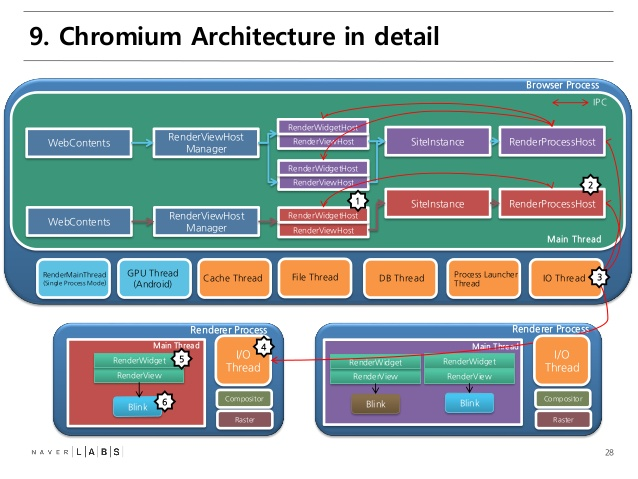
\includegraphics[scale=0.5]{figures/chromium-rendering-pipeline-28-638.jpg}
        \caption{Architectura de Chromium en detalle. Fuente: \cite{ChrRenderPipe}}
        \label{fig:archGC2}
    \end{figure}

    El \textit{Rendering Engine} usado por Google Chrome/Chromium, llamado Blink, es un \textit{forking} del trabajo original llamado Webkit. Su objetivo principal es soportar la architectura de multi-procesos que posee el navegador y al mismo tiempo poder reducir el nivel de complejidad. Cada nueva ventana o tab abre un nuevo proceso, y el Browser instruye a ese proceso a crear un componente que permitirá la visualización del recurso en el navegador. Cada proceso abierto para instanciar un Renderer estará en Sandbox, donde puede pasar que 2 tabs de diferentes dominios estén en el mismo proceso, dado que puede haber una relacíón en la navegación de éstas páginas.


    %     \begin{figure}[h!t]
    %     \begin{center}
    %         \includegraphics[scale=0.5]{figures/in_process_plugins.png}
    %       %\caption{Representación conceptual de una Nube con Eucalyptus. La especificación de las partes y su explicación se ve en \ref{sec:chap2.4.2}. Fuente \cite{EucalyptusOverview}}
    %       \label{fig:archG}
    %     \end{center}
    % \end{figure}

    %\subsection{Extensions}

    %\subsection{Plugins}
    %En el ultimo tiempo, los plugins como Adobe Flash

\section{Internet Explorer}
    \label{chap3:IE}
    Internet Explorer es el navegador grafico predeterminado por Microsoft y que su primera versión 1.0 fue realizada en 1995. IE es una derivación de Spyglass Mosaic desarrolado por la NCSA (National Center for Supercomputing Applications). En primera instancia fue un navegador que podría ser obtebido si era comprado como complemento de \textit{Microsoft Plus!} o mediante la versión \textit{OEM} de Windows 95. Desde la tercera versión de IE, en 1996, que esta se lanzó de forma gratuita.
            
    La arquitectura de este navegador es modular y permite al desarrollador por utilizar los recursos para crear diferentes funcionalidades, ejemplo de esto son: toolbars, Microsoft Active X controls, etc. En la Figura \ref{fig:archIE} \cite{IEArch} se puede ver los principales componentes de la architectura del browser mencionado. IE utiliza \textit{COM} o \textit{Component Object Model} una interfaz binaria standard para componentes de software introducida por Microsoft en 1993 y que permite una comunicación entre procesos/componentes de software provenientes de la familia de software de Microsoft. \textit{COM} es similar a otras tecnologías de interfaz de componentes de software ( Component Software Interface Technologies) cómo CORBA y Java Beans. El uso de \textit{COM} gobierna la forma la interacción de los componentes que se comunicann y permite que haya un reuso y extensibilidad de estos.
            
	\begin{figure}[h!t]
	    \centering
		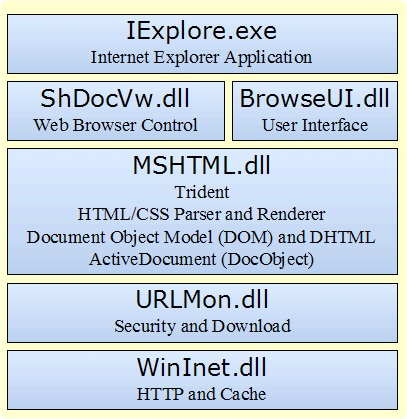
\includegraphics[scale=0.65]{figures/IEArch.jpg}
		\caption{Arquitectura de Internet Explorer. Fuente: \cite{IEArchImg}}
		\label{fig:archIE}
    \end{figure}

    \begin{figure}[h!t]
        \centering
        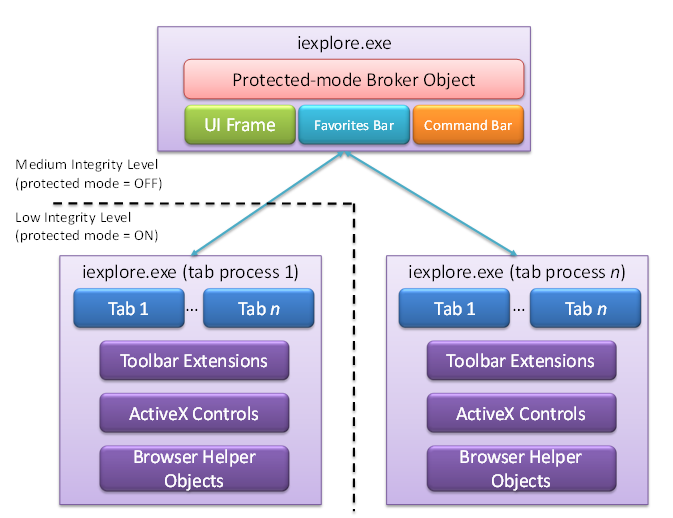
\includegraphics[scale=0.5]{figures/11_IE8andLooselyCoupledIELCIE_2.png}
        \caption{Arquitectura de Internet Explorer más detallada. Fuente: \cite{IE8LCIE}}
        \label{fig:archIE2}
    \end{figure}

    \subsection{Frame Process y Rendering Engine}   
        \label{chap2:Trident}
        O también llamado MSHTML, es un rendering engine privativo, sin embargo es posible usarlo al usar librería de Windows \textbf{mshtml.dll}. Según \cite{Crowley2010} es un objeto OLE (Object Linking and Embedding) Active Document que representa el \textit{layout} de Internet Explorer y permite mostrar graficamente las páginas por medio del \textit{display} del host. Dentro de éste se manejan las Extenciones, el \textit{engine} de Javascript y la librería que contiene la API para tareas de \textit{networking}, además de proveer una capa de seguridad y manejar las descargas de archivos.

    %\subsection{HBO}

    %\subsection{Plugins}


\section{Firefox}
    \label{chap3:Firefox}

    Firefox fue creado a partir del navegador \textit{Netscape} en 1998, actualmente la fundación Mozilla ha sido la que la ha mantenido, generando varias modificaciones desde su nacimiento. Las metas de diseño que Mozilla desee en el navegador son:
    \begin{itemize}
        \item Renderizado rápido de las páginas web.
        \item Fuerte apoyo a los estandares web como la W3C.
        \item Interoperabilidad en las diversas plataformas.
    \end{itemize}

    \subsection{Firefox Mono-proceso y Gecko}
        \begin{figure}[h!t]
    		\centering
        	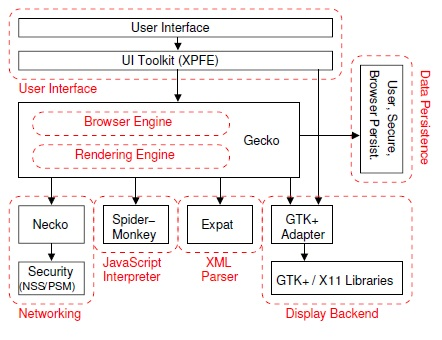
\includegraphics[scale=0.8]{figures/archMoz.jpg}
            \caption{Arquitectura Monoproceso obtenida en Fuente \cite{2005-grosskurth-browser-refarch, preprint-grosskurth-browser-archevol}}
            \label{fig:archM}
        \end{figure}
                
        La arquitectura de este browser puede ser vista en la Figura \ref{fig:archM} donde se pueden observar los siguientes componentes principales:
                \begin{itemize}
                    \item La interfaz de usuario, la cuál puede ser reutilizada para otras aplicaciones por su bajo coupling con el sistema entero. 
                    \item La persistencia de los datos, tanto de bookmarks como de data de bajo nivel como el \textit{cache}.
                    \item EL \textit{Rendering Engine}, permite el renderizado de documentos HTML/XML por un tipo de parser basado en web standardds. Este Engine es capaz de renderizar la interfaz de la aplicación multi-plataforma.
                    \item XPCOM
                \end{itemize}
        La arquitectura de Mozilla se distingue de las demás en que la visualización especificada por la plataforma y la librería de \textit{widgets} son usados directamente en el navegador, lo que minimiza el costo necesario para soportar diferentes plataformas. Si bien esta figura muestra lo más importante, algunos detalles relevantes son olvidados, como las extensiones y el componente XPCOM (cross, platform component object model) que es similiar al componente COM de Microsoft,

        Gecko es un motor de renderizado \textit{Open Source} que utiliza Firefox, escrito en C++, creado en un comienzo por Netscape, predecesor de Mozilla Foundation/Corporation. La función de este componente en Firefox (y otros browsers que lo integran) es leer el \textit{web content} de tipo HTML, CSS, XUL (para renderizar \textit{User Interface}) y Javascript, y mostrarlo al usuario en un formato gráfico. Tiene un gran rendiemiento al transformar a formato gráfico una página con lenguaje de marcado ya que soporta multithreading en el parser de HTML. Gecko fue diseñado para soportar \textit{Open Internet Standards} y por ende sigue al pie de la letra todas las especificaciones de HTML 4, CCS 1 y 2, DOM, XML y Javascript. Los componentes de Gecko incluyen:
            \begin{itemize}
                \item Parser de Documentos (HTML y XML).
                \item \textit{Layout Engine} con un modelo de contenido; ésta es la información que el display del host mostrará al usuario.
                \item Sistema de estilos.
                \item Motor de Javascript. En el caso de Gecko éste se llama \textbf{SpiderMonkey} que está escrito en C/C++.
                \item Librería de imágenes.
                \item Librería de \textit{Networking} o Necko.
                \item Renderizado gráfico específico a la plataforma y widget de acuerdo al sistema operativo.
                \item Librerías de Seguridad, NSS
                \item Mozilla Plug-in API (NPAPI).
                \item Lbrería de preferencias de usuario, entre otros más.

            \end{itemize}
        En la figura \ref{fig:Gecko} se explica como el Rendering Engine es capaz de crear una página a través de un HTML y su correspondientes CSS. Éste parte como 2 pipelines que leen tanto HTML como CSS, y cuando llegan al Frame Constructor se vuelven una. Ya en esa fase, se espera que solo una hebra se encargue del contenido visual que se mostrará, pues si se tuviera más habría problemas con las prioridades de los elementos a mostrar en el DOM y el Layout final.

        Finalmente, en el día de hoy los Plugins ya son considerados tecnología \textit{legacy}, en especial el uso de Adoble Flash, que estaba bien arraigado, ahora se ha empezado a utilizar HTML5 como una alternativa que se ajusta a los estándares de la W3C.

        \begin{figure}[h!t]
            \centering
            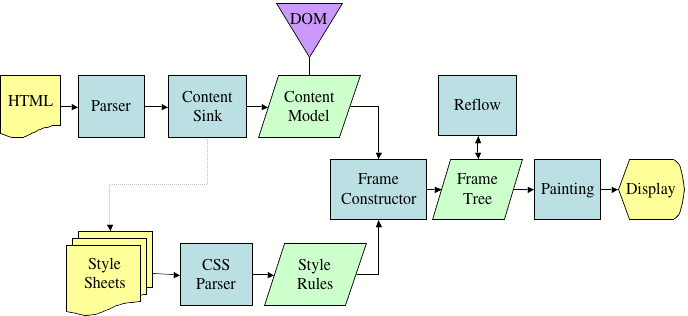
\includegraphics[width=0.8\textwidth]{figures/Gecko_Overview_9.png}
            \caption{Gecko Rendering Engine. Fuente: \cite{gecko}}
            \label{fig:Gecko}
        \end{figure}

        \subsubsection{Estabilidad y Recuperación a fallos}
        Este tipo de Firefox utiliza un proceso que se encarga de realizar tanto el Renderizado como la comunicación con las páginas web, y tiene la desventaja de que si sufre un fallo pequeño, todas las Tabs asociadas al proceso pueden ser corrompidas por el fallo. Así como también, el cierre inesperado puede causar una perdida total de los datos. Aunque Firefox sea uno de los Browser con mejor compatibilidad y sigue bastante bien los Web Standards de la W3C, le ha sido bastante dificil moverse a una arquitectura Modular como Google Chrome Y Explorer \cite{ElectrolysisTalk}
        
    \subsection{Firefox Multi-proceso (Electrolysis, e10s)} 
    Éste proyecto comenzó el 2009 y que por motivos desconocidos \cite{ElectrolysisTalk} se tuvo que poner en espera el proyecto. El 2012 la Arquitectura del Sistema Operativo Firefox empezó a usar la idea de multiprocesos que se había estado trabajando, por lo que el 2013 se recontinuó el proyecto, sin embargo aún no hay una versión estable y solo se puede ocupar como testing en la versión Nightly Build \cite{NightlyBuilds}. La nueva Arquitectura se basa en usar la aislación que provee el sistema operativo a los procesos, de la misma manera que lo hace Google Chrome, pero por supuesto el diseño no es el mismo.

    \subsubsection{Chrome Process y Content Process}
    Respecto a este componente de la nueva arquitectura que Electrolysis, no mucha información de que es lo que hace está en linea. Parte de los componentes son el sistema de comunicación que existe entre los procesos o Message Manager, que se encarga de enviar mensajes de control desde el Chrome Process a los procesos hijos o recibir los mensajes desde sus procesos hijos para realizar las acciones necesarias para mostrar el contenido.
        \begin{figure}[h!t]
            \centering
            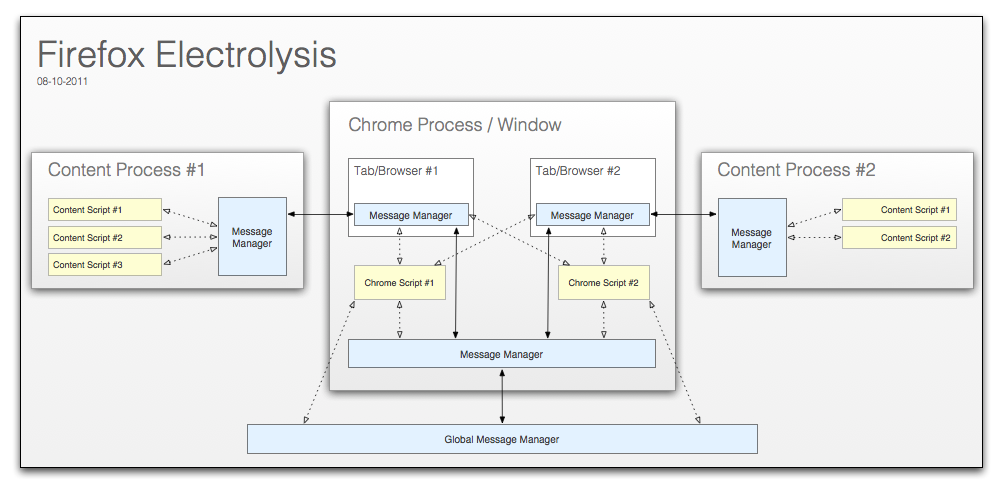
\includegraphics[width=0.8\textwidth]{figures/electrolysis.png}
            \caption{Firefox Electrolysis, communication 1. Fuente: \cite{Firefox101}}
            \label{fig:ChromePComm1}
        \end{figure}

    Así como Google e Internet Explorer, se tiene al Chrome Process como intermediario para cualquier tipo de acción dentro del Browser lo que permite controlar las peticiones del usuario o scripts que se ejecuten en el Content Process (hijo).

        \begin{figure}[h!t]
            \centering
            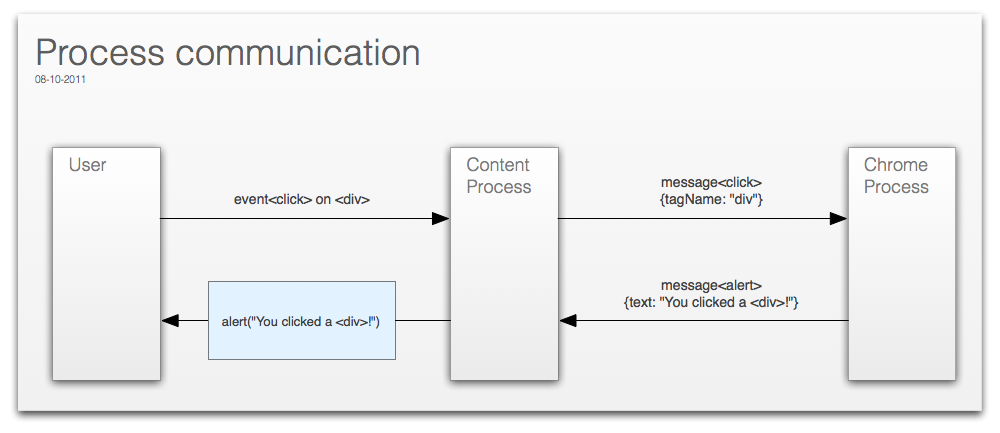
\includegraphics[width=0.8\textwidth]{figures/e10s-processes.png}
            \caption{Firefox Electrolysis, communication 2. Fuente: \cite{Firefox101}}
            \label{fig:ChromePComm2}
        \end{figure}

    Esta propuesta, si bien ha capturado buenas prácticas aún no ha podido realizar una implementación del Sandbox y está lejos aún.



\section{Mecanismos de Defensa del \textit{Browser}}

\subsection{Sandboxing}
    \label{chap3:Sandboxing}
    La idea es encapsular el área de mayor probabilidad de ataque en un espacio aislado, minimizando la superficie de ataque de un software. Sandboxing no es una técnica tan nueva, han existido sistemas que ya lo han incorporado. Ésta protección puede ser aplicada dependiendo del diseño del software, algunos ocupan Sandbox a nivel del sistema operativo como otros que ocupan al nivel del \textit{engine} de Javascript \cite{reis2009browser}. En el caso especial del \textit{Browser}, esta técnica es construida en el nivel más alto posible para un programa de usuario, lo que permite la separación de privilegios entregados por el sistema operativo al \textit{browser} y los subprocesos que corren dentro de éste. El atacante que se enfrente a un \textit{browser} que tenga este mecanismo de defensa, tendrá que realizar primero un \textit{bypass} encontrando una vulnerabilidad en el sandboxing del \textit{browser}. Existen diferentes técnicas para Sandboxing, todo depende del diseño del \textit{Browser}.

    En el desarrollo de \cite{barth2008security} se define un modelo de amenazas donde se enumeran las habilidades que debería de tener un atacante y los objetivos de estos, para así caracterizar y evaluar las propiedades de seguridad necesarias para evitar que los atacantes cumplan su objetivo. Una propiedad importante que hacen destacar en el estudio es cómo aislar ciertos procesos que pueden ser aprovechados por los atacantes y ofrece una forma para poder mitigar esto: Sandboxing. El Sandboxing de Google Chrome previene al atacante de leer o escribir en el sistema de archivos del usuario, dejando al Principal Web con los privilegios necesarios para parsear un HTML/XML y ejecutar código JavaScript. Sin embargo esta arquitectura no imposibilita al atacante a atacar otros sitios web si es que el Rendering Engine fue comprometido, lo que puede convertirse en una amenaza muy grande para otros sitios web.

    Mientras Google Chrome e Internet Explorer utilizan un Sandbox para sus procesos de Renderizado \cite{sandboxGC}, Firefox no ha realizado este trabajo siquiera en su versión monoproceso \cite{NeckoElectro}.



    \subsubsection{Google}
        El Sandbox de Google es una implementación propia y que también aprovecha las técnologías disponibles en el Sistema Operativo. La idea del Sandbox es restringuir el acceso o peticiones al sistema de archivos, de modo que la única manera es pidiendo a otro que realice el trabajo que el proceso dentro del Sandbox necesita.

        \begin{figure}[h!t]
            \centering
            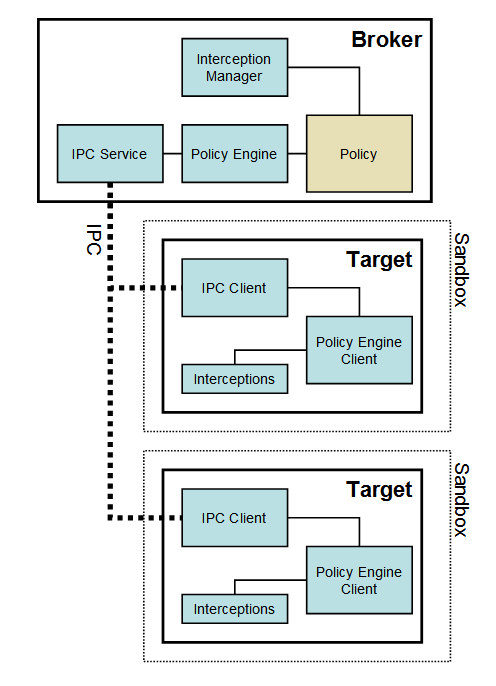
\includegraphics[scale=0.5]{figures/sbox_top_diagram.png}
            \caption{Sandbox interno de Google Chrome/Chromium. Fuente: \cite{sandboxGC}}
            \label{fig:SandboxGC}
        \end{figure}

    \subsubsection{Internet Explorer}
        Un nuevo mecanismo para aislar procesos es introducido en Windows 8, llamado AppContainer, es el principal mecanismo usado por Enhanced Protected Mode para aislar y limitar los privilegios y capacidades de un proceso con Sandboxing.
        \begin{figure}[h!t]
            \centering
            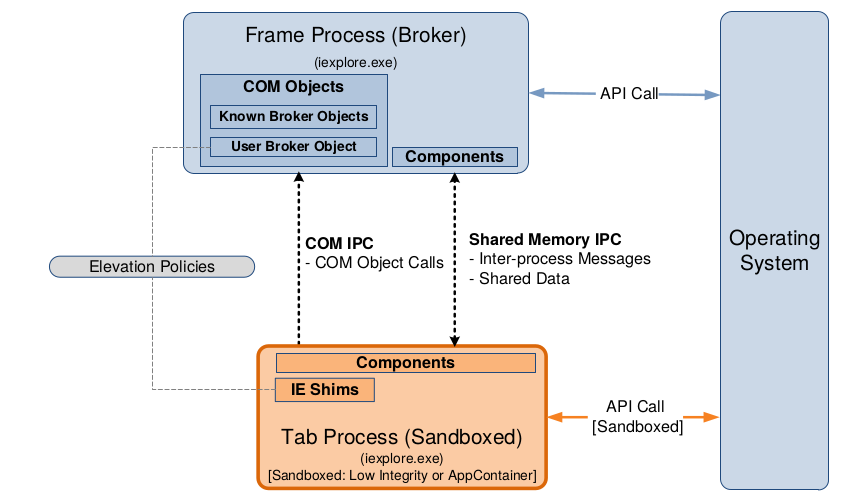
\includegraphics[scale=0.5]{figures/sandboxIE.png}
            \caption{Sandbox interno de Internet Explorer. Fuente: \cite{Yason}}
            \label{fig:SandboxIE}
        \end{figure}

        \begin{figure}[h!t]
            \centering
            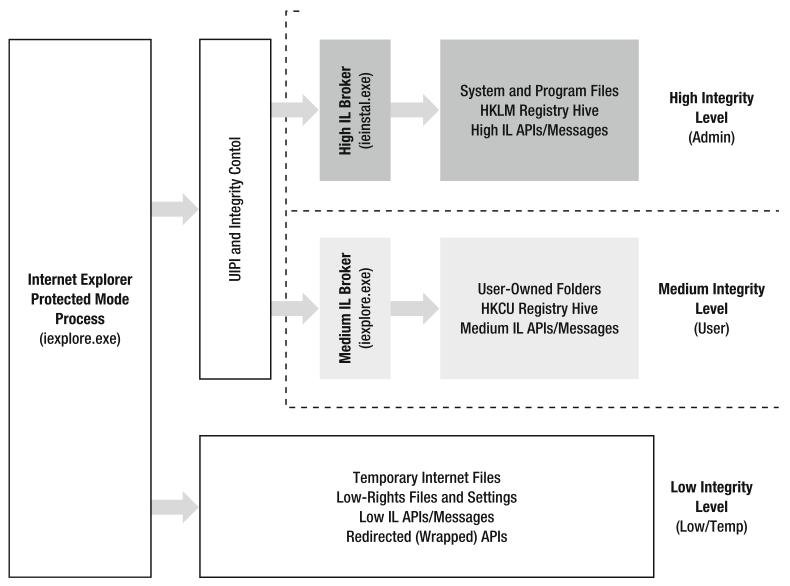
\includegraphics[scale=0.5]{figures/IEProtectedMode.jpg}
            \caption{Sandbox, Protected Mode. Fuente: \cite{Crowley2010}}
            \label{fig:SandboxIE2}
        \end{figure}
        La idea principal del Sandboxing en IE es restringuir el acceso de escritura a objetos \textit{asegurables}, como procesos, archivos o llaves de registro que sean de niveles de integridad mayor \cite{Colvin2010}. El proceso mismo de Internet Explorer posee un nivel de integridad baja, por lo tanto la única manera de modificar algo es cuando se le pregunta explicitamente al usuario y éste lo permite.



 \subsection{Aislación de Procesos}
    Cuando hablamos de Aislación de Procesos, nos referimos a cómo los Navegadores realizan la separación del contenido que será renderizada. Esto es dado que si no se es cuidadoso, scripts de otro \textbf{Origen} podrían intervenir con una página benigna y tomar control de ésta. Google Chrome aisla el contenido de cada recurso que el usuario pide, por medio de la instanciación de siteinstance-per-process \cite{Reis2009}, aunque durante este último tiempo están tratando de mejorarlo a site-per-process \cite{GoogleChromeIsolation}. Esto último significaría que cada página y frame tendría su propio proceso, separando completamente los espacios de memoria que cada componente de la página usaria al ser renderizada. Esto permite disminuir tanto la superficie de ataque, como incrementar la estabilidad del Browser, si es que algún componente provoca algún fallo. Firefox \cite{FirefoxThreatModel}, por su parte, promete que en futuras versiones del Browser multiproceso, diferentes Tabs podrán correr en diferentes procesos de acuerdo a su dominio, pero por ahora todas las tabs de contenidos comparten un solo process de Content process.

    La Aislación de Procesos es importante pues permite proveer de Seguridad, Sensibilidad, Estabilidad y Confiabilidad, pues al separar el proceso los espacios de memoria de cada procesos pueden ser random (si ALSR está activado \cite{Drake2011}). Además al separar en procesos, se están crendo distintas tareas que el sistema operativo se encargará de distribuir y computar de forma paralela. Y si alguno de estos procesos se cae, el proceso principal y todos los asociados, no deberían de ser afectados. Internet Explorer no indica que tipo de aislación provee en su documentación, pero debe ser algo entre lo que Google Chrome y Firefox proponen, pues los resultados que ellos han obtenido son alentadores.
    
    Uno de los pasos que ha tomado Google Chrome/Chromium y que Firefox va para el mismo rumbo con la API \textbf{WebExtension} \cite{AddONFirefox}, es la aislación de las extensiones del contenido de la página, tal como lo sugiere \cite{Barth2010}. Donde un Content script es el que podrá cambiar el contenido del DOM, pero no será capaz de afectar a las Tabs, Bookmarks de otro Tab y menos el sistema de archivos, a excepción que encuentre una vulnerabilidad que se lo permita.
    
    %GC: Barth2010, Barth2009SecureFrame, Reis2009, barth2008security
    %IE: Crowley2010, Yason
    %Todo: Drake2011, Saini2014, Silic2010

 \subsection{Blacklist y Whitelist de sitios web}

    El estudio \cite{browSecPhish} explica las más comunes y efectivas amenazas de seguridad que los usuarios hoy en día se enfrentan, entre ellas están el Software Engineering Malware y el Phishing. Un experimento es llevado a cabo en este estudio, con evidencia empiricamente validada y obtenida por NSS durante 12 días de continuo testing. Se obtuvo como resultado que Safe Browsing de Google Chrome provee una mejor protección contra ataques de tipo Phishing si es comparado con SmartScreen de Internet Explorer. Estos mecanismos poseen la habilidad para alertar a la posible víctima, de  que están a punto de pedir un recurso que puede ser malicioso. Una de las conclusiones del estudio \cite{rowSecSEMBlock} es que afirma que la tecnología de Google Safe Browsing no provee una protección adecuada para SEM, pero tecnologías basadas en CAMP ayudan bastante.

    Tanto Google como Firefox usan Safe Browsing para investigar si un cierto recurso, detrás de la URL pedida, es posible que se trate de un Phishing. Ambos tienen listas negras que se van actualizando muchas veces en el día, el menos 2 veces por hora. Esto permite disminuir la cantidad de ataques de éste tipo, pero lamentablemente el dinamismo de éste tipo de ataque a veces hace imposible tener una lista de todos los sitios manipulados.

    \cite{Rajab2013} utiliza una Whitelist dentro del cliente para limitar la cantidad de peticiones que se reciban desde todos los Navegadores que necesitan información sobre un binario, que posiblemente pueda o no ser un Malware.
        %GC y Firefox
    Internet Explorer utiliza URL Filtering, con el SmartScreen, que permite obtener una buena protección contra Social Engineering Malware \cite{rowSecSEMBlock} a diferencia de los otros manufacturados de navegadores.
    %\cite{Crowley2010, Colvin2010}

 \subsection{Sistemas de Reputación}
    %Agregar que estos s complementar con blacklist y a veces whitelist (GC)
    Cada vez que un usuario desea un recurso, por medio de su URL, el usuario podría no saber que detrás de ese \textit{path} puede haber una amenaza. Un sistema de reputación trabaja en base a los distintos tipos de binarios que un usuario podría llegar a descargar, ya sea un archivo muy descagado que podría estar disfrazado como una imagen y en verdad se trata de un virus, o simplemente un pdf que es descargado por un grupo de alumnos de un curso con poca concurrencia. La idea detrás es tener un sistema centralizado que se encarga de dar una \textbf{reputación} al binario, dependiendo de la técnica usada. Tanto Internet Explorer como Google Chrome utilizan este tipo de sistema, pero cada uno lo implemente de distinta manera. Un buen sistema basado en Reputación es aquel que es preciso y rápido, de manera que sea posible de obtener altos porcentajes de detección (efectividad).

    El estudio \cite{rowSecSEMBlock} realizado por NSS Labs, hizo una experimentación de la capacidad de detección y bloqueo de Malware en los Browser más conocidos, entre ellos Firefox, Internet Explorer y Google Chrome. Se usaron 657 muestras de Socially Engineering Malware o SEM (Malware basados en Ingeniería Social), que fueron capturados por el laboratorio dentro de 14 días. Los ataques basados en SEM usan diferentes métodos para poder engañar a los usuarios. Uno de los puntos que dejan claro, es que el fator primario es el Web Browser, dado que es la primera linea de defensa de los usuarios en contra de la mayoría de los ataques SEM. El test realizado dentro de la experimentación demostró que Internet Explorer bloqueaba casi un \(99,9\%\) de los SEM sacados de la muestra usadas dentro del test. Google Chrome le sigue a IE con la mejor detección de Malware y otros Browser con tecnologías basadas en Cloud (KingSoft Antivirus), generan una mejor detección que Firefox (\(4,2\%\)). La alta detección y bloqueo obtenido tanto por Internet Explorer y Google Chrome/Chromium, es gracias a las tecnologías SmartScreen URL Filtering (filtro de URL, como black list) y Application Reputation, Chrome por su parte usa Safe Browsing API y Download Protection para resguardarse. Sin embargo, Internet Explorer no depende tanto en su Sistema de Reputación así como lo realiza Google Chrome, donde el \(2,9\%\) del \(99,9\%\) de la detección de IE es basada en la técnología CAMP y Google Chrome detecta \(66,5\%\) del \(70,7\%\) con su Download Protection. Ésto último significa para Google Chrome/Chromium, que su sistemas de Reputación es su mejor protección contra Malware. 

    %\subsubsection{Google Download - Google Chrome/Chromium}
        %Ocupar referencias de NSS para los resultados obtenidos
    %\subsubsection{SmartScreen - Internet Explorer}


 %\subsection{Filtros XSS}
  %  Los Filtros XSS son una medida preventiva contra posibles ataques XSS insertados en la response del servidor. Principalmente se encarga de prevenir XSS de tipo Reflejado o Almacenado, pues los tipo DOM podría ocupar técnicas para 
    %Google e IE
    %Firefox ocupa 3rd party
    %Vulnerabilidades mencionadas \cite{Bates2010}y la solución del paper es crear un filtro que detenga los ataques antes de que sean interpretados por el Renderer
 %\subsection{Safe Sanitization}

 %\subsection{AdBlocker}

 \subsection{Actualizaciones Periódicas en Background}
 Tanto Google Chrome \cite{reis2009browser} como Firefox realizan actualizaciones automáticas periódicas del Navegador, para reducir la ventana de posible vulnerabilidades que pueda tener una versión. Parte importante de esto es que este proceso no fastidia al usuario y permite que se instale a penas el browser se cierra, para que en la próxima sesión sea posible usar la nueva.


% \subsection{Rendering Engines}
% \label{chap2:RenderingE}
% Responsable de converitir la página web, en HTML o XML, a un formato visible cómodo para el usuario en la pantalla del host. La combinación de HTML, CSS y media (imagenes, videos, etc.) permiten entregar una experiencia gráfica al usuario con la que interactuará. Existen browser que no usan gráficos y solo se basan en mostrar texto, ejemplos de estos navegadores son: W3M y Lynx. Los \textit{Rendering Engines} más usados son: Webkit (Safari), Blink (Google Chrome/Chromium), Trident (Internet Explorer) y Gecko (Firefox).

%     \subsubsection{Trident}
%     
%     







